\chapter{Supernova cosmology}

We want to use the relationship between the apparent brightness and the known (or calibrated) luminosity of objects to measure the cosmological model through the luminosity distance $D_L(z)$, ultimately depending on the expansion history $a(t)$.  Type Ia supernovae are luminous and fairly consistent explosions of white dwarf stars and have been the workhorse for cosmological measurements of this type.  They are complicated objects, not understood from first priciples, but are well-characterized and standardized.  In the following, we will describe the supernovae and the Cepheid variable-type stars used to calibrate their luminosities.  We will examine in detail measurements of photometry and spectra made in an expanding universe.  These are the necessary data.  Then we will see how researchers build a statistical model of the Type Ia spectral energy distribution and finally how this used to make a calibrated distance estimate for each object.  The statistical methods to fit for the cosmomology have to wait for the next chapter.


\section{Distance ladder}
Many Type Ia supernova have been studied in detail with photometric time series of their brightness, so-called ``light curves,'' in multiple spectral bands.  A smaller subset have had more costly spectroscopic measurements to characterize their full spectral energy distribution.  Despite this effort, that information cannot on its own tell us how luminous the explosions are.  None are close enough for a direct geometric measurement of their distance.  We need to calibrate them with another type of object, usually Cepheid variable stars.  Some Cepheids are near enough to us to know their luminosities by comparing their measured brightness to their distance measured geometrically and precisely via parallax, using the Earth's orbit around the Sun.  By extrapolating those results to Cepheids bright enough to see in intermediate-distance galaxies that also hosted a Type Ia supernova, we can determine the distances to those galaxies and calibrate the luminosity of the Type Ia class of objects.

% Using nomeclature of 2025arXiv251023823H
Thus to build a ``ladder'' to the distant Universe, we are using parallax measurements of the Milky Way Cepheids to anchor the calibration for the Cepheids and allow us to use extragalactic cepheids as a primary distance indicator in our distance ladder.  This allows us to determine distances to the galactic hosts of supernovae and calibrate the supernovae as secondary distance indicators \citep{2025arXiv251023823H}.


\textcolor{red}{There are other primary distance indicators and other possible geometric anchors.  TRGB, surface brightness fluctuations, maser, etc.}

detached eclipsing binaries (DEB),

A handful of galaxies have been discovered that contain masers in the accretion disk at the central black hole.  An astrophysical maser is like a natural microwave laser, a two-level system where an inverted population generates intense stimulated  monochromatic line emission, but without a resonant cavity.  A 


the Tip of the Red Giant Branch (TRGB),
Miras,
carbon-rich AGB stars (JAGB),

Other secondary distance indicators include
Surface Brightness Fluctuations (SBF),
Type II supernovae (SNe II),
the Fundamental Plane, and
Tully-Fisher relations



\subsection{Type Ia supernova} % What is a SNIa?

\begin{figure}
  \begin{center}
        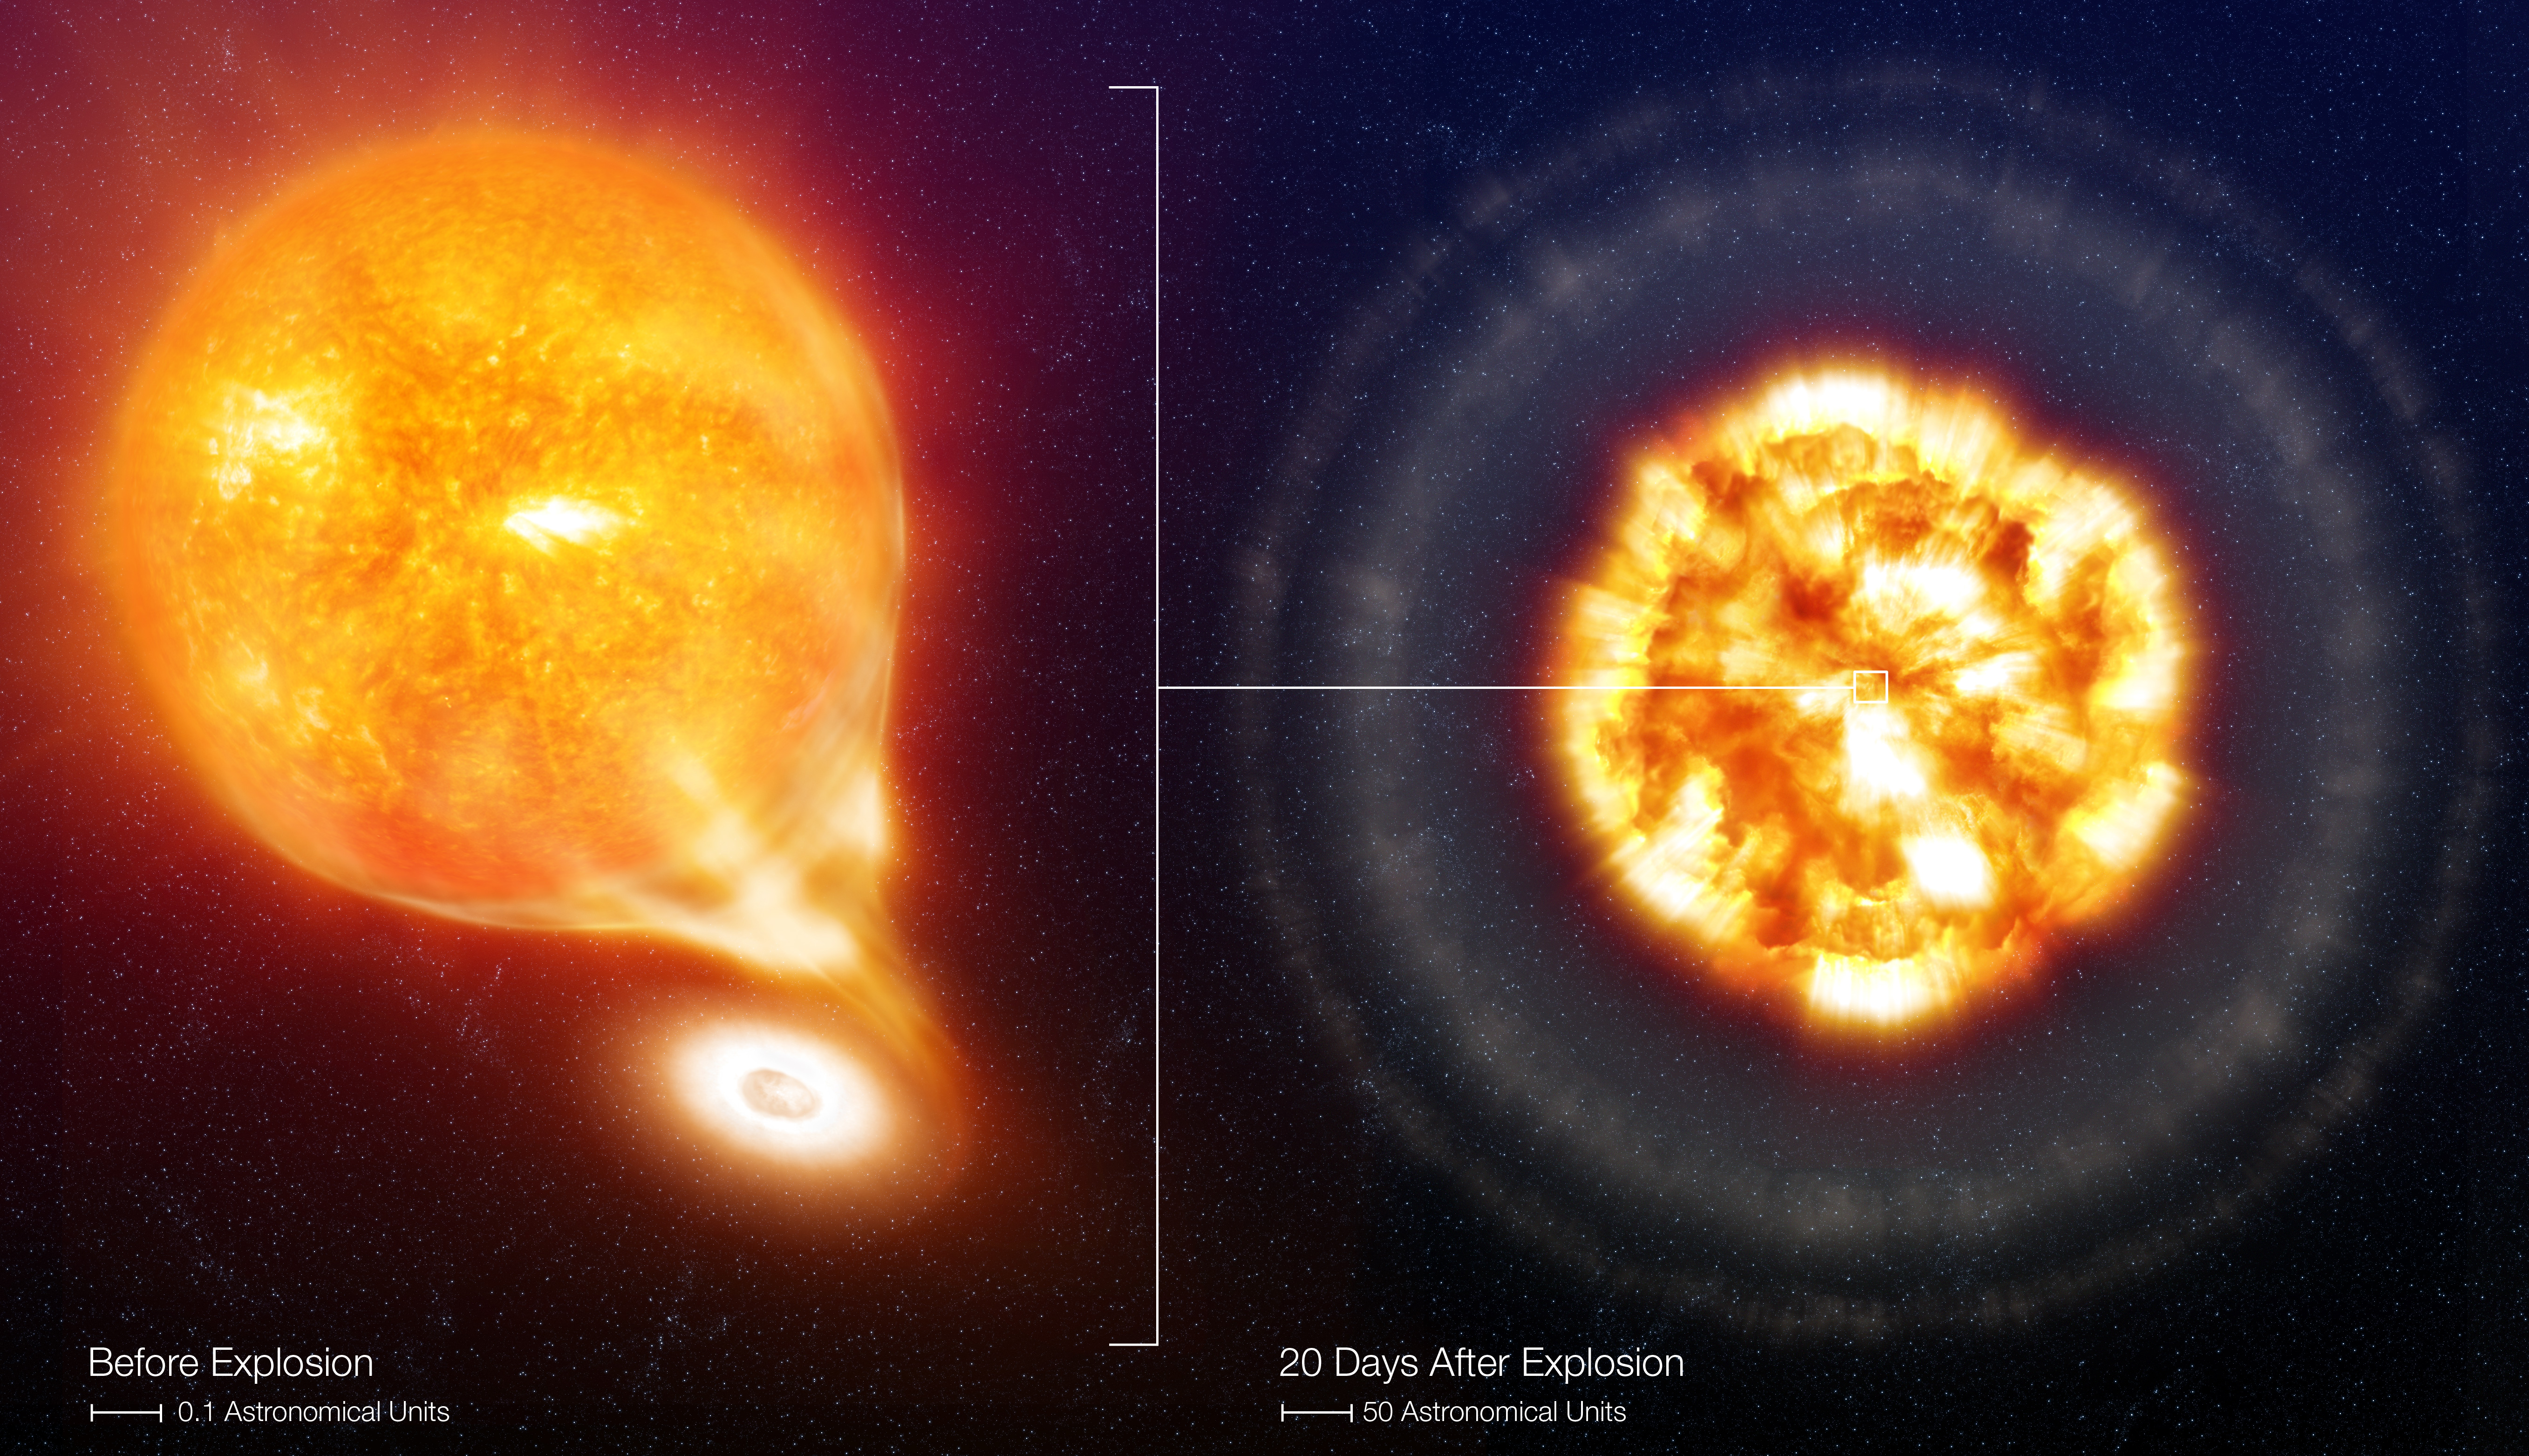
\includegraphics[height=4.3cm]{figs/standard_candles/SN_2006X,_before_and_after_the_Type_Ia_Supernova_explosion_(artist's_impression).jpg}
\hfill
    \includegraphics[height=4.3cm]{figs/standard_candles/SN_1006.jpg} % https://commons.wikimedia.org/wiki/File:SN_1006.jpg
  \end{center}
\caption{Left and center:  before a Type Ia explosion, in an artist impression of the single-degenerate scenario, an evolved giant star donates material to the small white dwarf, eventually triggering an explosion.  After $\sim 20--30 days$, the photosphere of the reaches its maximum luminosity.  Right: the nearly-spherical remnant of historical SN 1006, 1000 years after the explosion, seen by Chandra telescope in three bands of x-rays and thought to be a Type Ia supernova in the Milky Way galaxy.  The diameter is about 19 pc or 4.0 million AU.  There is no clear candidate for the companion, so this supernova may have formed in a double-degenerate (two-white-dwarf) collision that was completely disrupted.}
\end{figure}

A Type Ia supernova is the catastrophic nuclear explosion of a white dwarf star.  White dwarfs are the evolutionary endpoint for the cores of low-to-medium mass stars, under about 8 solar masses.  Most of these stars are composed of carbon and oxygen, having burnt hydrogen to helium during their main sequence lifetimes.  They proceeded to swell transiently up as red giants, and then burnt the core helium to carbon and oxygen as a horizontal branch star.  After swelling again to form asymptotic giant branch stars, the stars shed the outer layers to leave the bare cores.  A typical white dwarf is similar in size to the Earth (radius $\sim 6000$ km) but contains $\sim 1$~$M_\odot$ of material, yielding a density $\sim 10^9$ kg/m$^3$.  Counterintuitively, more massive white dwarfs are smaller, compacted by their strong gravity to higher density.  The core of a white dwarf is not fusing, and rather than being supported by the gas pressure from its temperature, it is supported by the degeneracy pressure of the dense electrons which, following the Pauli exclusion principle, pile up to fill all the lowest energy states up to the Fermi level.

White dwarf stars have a maximum mass, about 1.4 $M_\odot$ for a non-rotating star, the Chandrasekhar limit\index{Chandrasekhar limit}.  Above that, electrons even in the lowest available energy states become relativistic, provide a softened equation of state, and are unable to support the core against collapse.  Before the core reaches that point, however, the increasing density triggers a thermonuclear detonation of the carbon fuel, powering the explosion.  This is the difference between the carbon-oxygen white dwarf's thermonuclear supernova and the core-collapse supernova of a higher-mass star, where the core has already burned to iron and there are no more exothermic fusion reactions once the electron pressure gives out.  The thermonuclear explosion disrupts the white dwarf, typically leaving no compact remnant,\footnote{An exception is the rare subtype Iax, where the supernova leaves behind a fragment of the white dwarf, known as a zombie star.} while a core-collapse supernova will leave behind a neutron star or black hole.

Where does the white dwarf get the extra mass to explode?  There are two main pathways.  In the single-degenerate-progentior model, the star starts in a binary system of two main sequence stars.  The more massive, primary star evolves quicker and forms a giant star first, temporarily enveloping the secondary star in a process that ejects mass and angular momentum and reduces the orbital radius, then proceed to form the white dwarf star.  Later, the second star evolves and swells to a giant, allowing the white dwarf to capture and accrete the tenuously-held outer layers.  A white dwarf that explodes with this mechanism will always be smaller than the Chandrasekhar mass.  These account for perhaps fewer than 20\% of Type Ia supernovae.

In the double-degenerate-progenitor model, the explosion comes from two white dwarfs colliding.  This could happen in a dense star cluster, or in a binary system disrupted by the close passage of a third star or another binary system; the collision of isolated stars is possible but too rare to account for the Type Ia rate.  A close binary of white dwarf stars will have its orbit decay via gravitational radiation.  Once the stars merge, the mass before the imminent explosion may exceed the Chandrasekhar limit.  The double degenerate scenario is favored for most Type Ia supernova because of the lack of suitable companion stars in Type Ia supernova remnants, and because of the lack of observed X-ray emission in active supernovae, which would result from the interaction of the explosion and a companion's outer layers.  The numbers of observed binary white dwarfs are also in line with the observed rate of Type Ia supernova, about  $0.55^{+0.50}_{-0.29}$ (stat.) $\pm 0.20$ (sys.) Mpc$^{-3}$ year$^{-1}$ \citep[][]{2015A&A...584A..62C}, or about 1 supernova per century in a Milky Way-sized galaxy. 

The exact explosion mechanism inside the white dwarf is an area of active research. As the nuclear burning front moves through the star, it could be subsonic (a deflagration) or supersonic (a detonation).  A pure deflagration model is disfavored because the slower burning allows the star to expand and adjust to the changing temperature and pressure, resulting in a less luminous explosion and paucity of burned products. A pure, supersonic detonation is also disfavored because it traverses the star before the star can react hydrodynamical, and yields a near totally complete burning of the carbon-oxygen fuel to iron group elements (iron, nickel, and cobalt).  The currently favored model starts with a deflagration that expands and mixes the star slightly followed by a detonation, which yields the appropriate amount of intermediate mass elements (like silicon, sulfur, and calcium) and iron group elements.  Another model experiences a detonation in an exterior shell of helium that sends a shock wave into the interior, triggering the main detonation deep inside.  Different mechanisms may be at play in different explosions.  The energy released within a few seconds by the nuclear fusion is sufficient to unbind the star.

\begin{figure}
  \begin{center}
    \includegraphics[width=0.49\textwidth]{figs/standard_candles/SNIacurva.png} % https://commons.wikimedia.org/wiki/File:SNIacurva.png
    \includegraphics[width=0.5\textwidth]{figs/standard_candles/stretch_correction.jpg} % Figure 1 from 2003PhT....56d..53P
  \end{center}
\caption{Left: Light curve of a type Ia supernova, the initial peak powered by radioactive nickel, followed by a long tail of emission from radioactive cobalt which has a longer half-life.  Right: stretch-correcting the light curve and peak luminosity \citep[from][]{2003PhT....56d..53P}.} \label{fig:Ia_light_curve}
\end{figure}

Matter is ejected in an expanding shockwave at 5,000--20,000 km/s.  As the density of the outer layer falls, the photosphere become optically thin, successively revealing interior layers with different compositions and yielding a complex spectral behavior.  The explosion creates radioactive $^{56}$Ni in abundance.  With a 6.1 day halflife, this beta decays to $^{56}$Co. The peak luminosity and susequent fading from the peak is powered by this radioactive nickel (Figure~\ref{fig:Ia_light_curve}).  The resulting $^{56}$Co beta decays to stable $^{56}$Fe with a 77.2 day halflife.

The more $^{56}$Ni produced, the more luminous the supernova.  Empirically, the more luminous light curves\index{light curve}---time-series of photometric brightnesses---are broader; they take more time to peak and decline (also Figure \ref{fig:Ia_light_curve}).  Supernova with greater nickel abundance have higher temperature and more highly ionized gas, which leads to higher opacity and a longer photon-diffusion timescale, so they glow for more time.  As iron group ions recombine, they produce overlapping absorption lines, particularly in the UV and blue end of the spectrum.  The hotter, more luminous supernova (with more $^{56}$Ni), where this recombination is delayed, tend to be bluer, and decline slower in the blue B band where the analysis is typically normalized.

Spectroscopy is far more time intensive than photometry, and ``Type Ia'' was originally an observational, spectral classification.  Because the progenitor is a carbon-oxygen-rich object, having shed the outer layers, the supernova shows no hydrogen lines, making it a Type I instead of a Type II that shows hydrogen lines.  Type Ia spectra show an absorption feature from silicon, one of the intermediate mass fusion products, while the other Type I supernovae, Ib and Ic, lack this line.   (These are core collapse supernova of more massive stars that have shed their hydrogen or hydrogen and helium layers before exploding.  Accordingly, Type Ib include helium lines and Type Ic lack them.)  Type Ia can also be distinguished by photometry alone, from their unique nickel-to-cobalt light curve.


At the date of this writing, the most distant Type Ia supernova is at redshift 2.9, seen in the first two years of JWST \citep[SN 2023adsy,][]{2025A&A...701A..70V}, although this will likely be surpassed soon.  The total number of well-measured Type Ia supernovae that are included in cosmological analysis is somewhat less that \textcolor{red}{2000}.  These require multiband light curves to characterize the maximum brightness and estimate the main corrections to the luminosity, the light curve timescale and the supernova color.  The number of supernovae with Cepheid-calibrated distances, and thus some notion of their intrinsic luminosity, is also not large, perhaps under \textcolor{red}{70}.

\subsection{Cepheid variables}


Type II Cepheid stars are luminous (absolute magnitude $M \sim -1$ to $M \sim -5$ versus $M = +4.83$ for the Sun) and common enough in the Milky Way that we can calibrate the period--luminosity relation via geometric parallax in the Gaia data.

NGC 4258 helped with the calibration of cepheids because it has a broader range of metallicities than overlaps both with the milky way and other galaxies.


  The numbers of anchor objects is not large fewer than \textcolor{red}{100} by parallax in the Milky way. 

Maximum distance that we can see a cepheid?

  
\section{Point sources of radiation}

We can characterize the brightness of an object by its spectral flux density, which tells you how much energy per time you would collect from that source in unit collecting area within a unit bandwidth of the radiation spectrum.  

Looking at the definition of flux density and its units, it is clear that in order to figure out how much energy $E$ you would receive from an object during an observation, you need to integrate the flux density $f_\lambda$ over the time of observation $dt$, collecting area $dA$, and bandwidth $d\lambda$.
\begin{equation}
  E = \int f_\lambda \, dt\, dA\, d\lambda
\end{equation}
The units for brightness are thus $\mbox{W m}^{-2}\mbox{ m}^{-1}$ where the  m$^2$ corresponds to area and the m corresponds to wavelength.
If the detectors are not equally efficient at every frequency or over all parts of the receiver's collecting area, in practice you need to multiply the flux density by efficiency factors that are a function of position or frequency before integrating, such as
\begin{equation}
  E_{\rm band} = \int R_{\rm band}(\lambda) f_\lambda \, dt\, dA\, d\lambda
\end{equation}
where $R(\lambda$) is the efficiency of the detector/filter combination, which ranges from zero to one.
Here we have assumed that we are describing the spectrum in terms of the wavelength  of the radiation (common in optical astronomy), but this could equivalently be done in terms of the frequency of radiation (common in radio astronomy).  If we think of
\begin{equation}
   f_\lambda = \frac{dE}{dt \, dA \, d\lambda}
\end{equation}
as we have done above, or alternatively,
\begin{equation}
  f_\nu = \frac{dE}{dt \, dA \, d\nu}
\end{equation}
then it becomes clear that
\begin{equation}
  f_\nu = f_\lambda \left| \frac{d\lambda}{d\nu} \right| = f_\lambda \frac{c}{\nu^2} = f_\lambda \frac{\lambda^2}{c}
\end{equation}
where we have used the speed of light and the relation $\lambda = c/\nu$ in the last equations.  Even though $\lambda$ decreases when $\nu$ increases, so the derivative is negative, by convention we make both spectra $f_\nu$ and  $f_\lambda$ positive, which accounts for the absolute value.

We don't receive much power from astronomical objects.  In radio, microwave, and sub-millimeter band astronomy, the typical unit for brightness is called the Jansky, which in SI units is
\begin{equation}
  1\ \mbox{Jy} = 10^{-26}\ \mbox{W m}^{-2}\mbox{ Hz}^{-1}
\end{equation}


We can model the contribution of a point source to the sky signal as a delta function:
\begin{equation}
  s_\lambda(\hat n) = f_\lambda \delta( \hat n - \hat n_0)
\end{equation}
where $\hat n$ is a direction on the sky and $\hat n_0$ is the vector that points to the source of radiation.  If we thus integrate any area of sky (or \textit{aperture}) that contains the source, we get the value $f$ of its brightness. Note that the delta function  on the two-dimensional sky has units of inverse angle squared, or inverse solid angle. 

Of course, telescopes do not have perfectly sharp imaging, and so radiation coming from one direction is detected from other, nearby directions.   Light from a single direction spreads out onto the focal plane, falling into several pixels on the camera.  This effect of the telescope's resolution we call this the ``point-spread function'' in optical or infrared astronomy, because it describes how a point of light is spread out on the image. In radio and microwave astronomy, we call the same thing the telescope ``beam,'' because if you reverse the purpose of the radio dish, and use it as a transmitter instead of a receiver, the point-spread function describes intensity of the beam of radiation that the horn or dish puts out as a function of angle to the telescope boresight.  The original delta function of radiation gets convolved to produce the image of surface brightness captured by our camera exposure.

We will continue a detailed discussion of the point spread function or beam in the section on the cosmic microwave background, where it figures into an important correction for the measurement of fluctuations.  For now we will assume that we can get good photometry, a good measurement of the brightness, by integrating up the light from the star or supernova as it is spread by the optics across several pixels.

Thus the bolometric brightness of the object, which occurs in the luminosity distance, is
\begin{equation}
  F = \int_{{\rm all}\ \lambda} f_\lambda d\lambda 
\end{equation}
or
\begin{equation}
f_\lambda = \frac{dF}{d\lambda}
\end{equation}
while the flux in a band, is
\begin{equation}
  F_{\rm band} = \int R(\lambda) f_\lambda d\lambda = \int R(\lambda) s_\lambda d\lambda d\Omega. \label{eqn:flux_in_band}
\end{equation}
using the band filter function $R(\lambda)$. It is straightforward to make similar expressions employing $f_\nu$.

The band-averaged flux density is
\begin{equation}
  f_{\rm band} = \frac{\int R(\lambda)  f_\lambda d\lambda}{\int R(\lambda) d\lambda} = \frac{F_{\rm band}}{\int R(\lambda) d\lambda} 
\end{equation}
which is just a weighted average of $f_\lambda$ over the band.  This has the advantage of giving roughly the same value if the band is not too wide compared to features in the spectrum and will give similar values for moderate differences in the band.  You can also think of the effective wavelength of the band for a particular spectrum of source
\begin{equation}
  \lambda_{\rm band} = \frac{\int \lambda R(\lambda)  f_\lambda d\lambda}{\int R(\lambda)  f_\lambda d\lambda} = \frac{\int \lambda R(\lambda)  f_\lambda d\lambda}{F_{\rm band}}
\end{equation}
which is like the mean wavelength or a first moment of the spectral/band distribution.  Unless the spectral/band combination is multimodal, this will be the wavelength near where the flux density equals the band-averaged flux density.

\begin{figure}
  \begin{center}
    \fakeplot
  \end{center}
  \caption{Filter functions of photometric systems. Nice to show UBV and ugrizy.}
\end{figure}

Every telescope has its own filters and wavelength response that define its bands.  Some notable photometric systems include the Johnson UBV system, Rubin-LSST ugrizy, and SDSS u',g',r',i',z'.  Hubble Space Telescope's WFC3 and James Webb Space Telescope's NIRCam have filters named for their central wavelength and shape, for example NIRCam's F150W, a  band centered at 1.5 $\mu$m that is 0.4 $\mu$m ``wide,'' wider than the other bands at the same wavelength.


\subsection{Magnitude system}
I am no great fan of it, but it is common in astronomy to use the traditional 19th-century logarithmic system of \textbf{stellar magnitudes}\index{magnitude system} to describe the brightness of objects.  Magnitude systems have two properties.  First, if two fluxes are in a ratio of 100, they will differ by 5 magnitudes, with the brighter having the \textit{lower} magnitude.  This connects back to the 2000-year-old visual star catalog of Greek astronomer Hipparchus (and popularized by Ptolemy) who ranked the brightest stars as first magnitude, the next brightest as second magnitude and so on.  The second property sets the zero point for the magnitude scale and warrants more discussion below.

The relationship between fluxes and magnitudes is thus
\begin{equation}
  \frac{F_1}{F_2} = 100^{(m_1-m_2)/5},
\end{equation}
or equivalently,
\begin{equation}
  m_1-m_2 =  -\frac{5}{2} \log_{10} \left( \frac{F_1}{F_2} \right).
\end{equation}
Here $m_1$ and $m_2$ are called apparent magnitudes because they are based on the brightness that is apparent to our observation.

Although the magnitude carries the same information as the flux, and perhaps adds some unnecessary confusion, the magnitude system does ease the job of calibrating the photometry in the following sense.  It is straightforward to get relative calibration for a target object by comparing the ratio of its brightnesses to a calibration star in the same image with a known magnitude.  Any multiplicative calibration factors inherent to that particular image divide out, like the time of exposure or efficiency of the detector.  If no calibration star is available, the magnitude calibration can be chained back, bright star to bright star, to one of known brightness though several links.  For calibration, it's only straightforward to compare two fluxes of alike types, for example, two bolometric fluxes or two g-band fluxes.

There are two common choices of normalization or zero point, stellar-based or absolute.  The normalization can be thought of as choosing a reference flux in the band
\begin{equation}
  m_{\rm band} = -2.5 \log_{10} \left( \frac{ F_{\rm band}}{F_{{\rm ref},\ \rm band}} \right) = -2.5 \log_{10} \left( \frac{ f_{\rm band}}{f_{{\rm ref},\ \rm band}} \right) ,
  \label{eqn:reference_flux}
\end{equation}
(equal because the band-averaged $f$s have denominators that cancel) or equivalently an additive constant in
\begin{equation}
  m_{\rm band} = -2.5 \log_{10} \left( \frac{ F_{\rm band}}{[\mbox{flux unit}]} \right)  + C_{\rm band}.
\end{equation}
The Vega magnitude system chooses these references so that the magnitude of the star Vega is zero in all bands, using $F_{{\rm ref},\ \rm band} = F_{{\rm Vega},\ \rm band}$.  Vega, a spectral type A0 star with blackbody temperature about 8,900 K, is a slightly problematic choice for precision work since it is variable by about a tenth of a magnitude.  The similar Johnson UVB system defines zero magnitude in each band with the average of six stars with the same spectral type as Vega.

The AB magnitude system, on the other hand, provides an absolute energy calibration without depending on particular stars.
For any bandpass filter, it is defined so that
\begin{eqnarray}
  m_{AB} &=& -2.5 \log_{10} \left( \frac{\int R(\nu) f_\nu d\nu}{\int R(\nu) (1\mbox{ Jy})  d\nu} \right) + 8.90 \\
  &=&  -2.5 \log_{10} \left( \frac{\int R(\nu) f_\nu d\nu}{\int R(\nu) (1\mbox{ erg s}^{-1}\mbox{ cm}^{-2}\mbox{ Hz}^{-1}) d\nu}  \right) - 48.60, \nonumber
\end{eqnarray}
or
using a reference flux in equation \ref{eqn:reference_flux} of
\begin{equation}
  F_{{\rm ref,\ band}} = \int R(\nu) (1 \mbox{ Jy} \cdot 10^{-8.90/-2.5}) d\nu \approx \int R(\nu) (3631 \mbox{ Jy}) d\nu.
\end{equation}
Note that $f_\nu = 3631$ Jy is close to the flux density of Vega in V band (but not other bands) and is the reason that value was chosen.  AB magnitudes make a pretty good definition because it puts the scale on firm footing with respect to energy units.\footnote{Note that these expressions are sometimes written for a very narrow filter over which the $f_\nu$ doesn't vary, and the integral $\int R(\nu) d\nu$ is canceled on top and bottom, leaving only e.g.\ the $(f_\nu/1\mbox{ Jy})$ in the logarithm and defining a monochromatic magnitude rather than a band magnitude.  Sometimes the units are left out of the equation entirely, but mentioned in text instead, which I think is a confusing abuse of unit notation.  Other times, the filter function is written as $R(\nu) =  p(\nu) (h\nu)^{-1}$ where $p(\nu)$ is the ``capture cross section'' that quantifies the probability of counting an incident photon as an $e^-$ in the detector.  The $h\nu$ is the energy of that photon to convert between the fraction of photons getting through and the fraction of energy getting through.  It helps to pay careful attention to these definitions when you encounter a bandpass function.}
To actually get this you still have to go through a chain of calibration, typically using standard stars along the way.

A \textbf{color index}\index{color index} difference between the magnitudes in two bands, like $m_B-m_V$ (often written a simply $B-V$), is a comparison of the received energy flux between the bands.  In a Vega-based magnitude system, it is the base-10-logarithm of that ratio divided by the similar ratio from Vega.  Thus stars with the same spectrum as Vega have color indices equal to zero for all pairs of bands.  Across the visual bands, for smaller wavelength magnitudes minus larger wavelength magnitudes, the color index is negative for stars hotter than Vega and positive for stars cooler than Vega.

One disadvantage of the magnitude system is that it becomes difficult to add or accumulate.  
Two 10.0 magnitude stars in binary system add to a total magnitude of 9.25 while two 20.0 mag stars add to a total of 19.25 because the decrease $\Delta m = -0.75$ corresponds to a doubling
of flux.
The common practice of providing surface brightness with a unit of mag/arcsec$^2$ is really terrible.  It means that a 1 arcsec$^2$ pixel would have a flux corresponding to the particular magnitude (regardless of the actual pixel size), but these must be converted back to flux to add up the flux.

For supernova cosmology analysis, it is important to bring all the varied photometry of various supernova over the year to a common photometric system, which entails a multitude of telescopes and filters with secondary and tertiary stars common between various surveys to be compare and modeled \citep{2022ApJ...938..111B}.  Reliable photometry is vitally important and a lot of work.

\subsection{Distance modulus}
While the apparent magnitude measures the brightness of an object, the \textbf{absolute magnitude}\index{absolute magnitude} measures its luminosity.  The absolute magnitude $M$ is defined as what the apparent magnitude would be if we imagine the object were 10 pc away.\footnote{Absolute magnitude was conceived for stars and is kind of inappropriate for a supernova, since a supernova at 10 pc would be exceedingly dangerous, destroying the ozone layer and causing a mass extinction on Earth.}  Considering bolometric magnitudes, 
\begin{equation}
  100^{(m_{\rm bolo}-M_{\rm bolo})/5} = \frac{F_{10\ \rm pc}}{F} = \frac{{L}/{4\pi(10\ \rm pc)^2}}{{L}/{4\pi D_L^2}} = \left( \frac{D_L}{10\ \rm pc} \right)^2
\end{equation}

The apparent magntitude we can measure and so it is easier to get than the distance or absolute magnitude.  In cosmology, we are often trying to learn the absolute magnitude or the luminosity in order to determine the luminosity distance as a function of redshift and thus the cosmology.


\begin{figure}
  \begin{center}
    \fakeplot
  \end{center}
  \caption{Distance modulus vs. redshift, with or without SNIa data.}
\end{figure}

Taking the logarithm yields the \textbf{distance modulus}, a measurement of luminosity distance that equals the difference between the apparent and absolute magnitude.  

\begin{equation}
  \mu \equiv   5 \log_{10}(D_L / 10\,\mbox{pc}) =  m_{\rm bolo} - M_{\rm bolo}
\end{equation}

In a band, the absolute magnitude is
\begin{eqnarray}
  M_{\rm band} &=& -2.5 \log_{10} \left( \frac{F_{\rm band,\ 10 \ pc}}{F_{\rm ref, \ band}}  \right)  \\
  &=&   -2.5 \log_{10} \left( \frac{ \int R(\lambda) f_{\lambda,\ 10\ \rm pc}\ d\lambda}{F_{\rm ref, \ band}} \right).
\end{eqnarray}
For the Sun, $M_V = +4.83$ while $m_V = -26.7$.  For Type Ia supernova $M_V \sim -19$.

\subsubsection{Reddening}
$E(B-V)$ actually means $(m_B - m_V)(\hat \mathbf{n})$, magnitude difference due to dust reddining as a function of position on the sky.

Milky Way reddening

reddening in the host galaxy.

\subsection{K-corrections}
When you measure an object at high reshift in a filter band, relevant here for cosmology, you must make a further correction.  The emission that you receive is redshifted from that which was emitted and the wavelength increment in the bandwidth is also redshifted.  To compute this correction, let's recall that observed wavelength relates to the emitted wavelength as
\begin{equation}
  \lambda = (1+z) \lambda_{\rm em}.
\end{equation}
Then, for the spectral flux density we will have,
\begin{eqnarray}
  f_\lambda = \quad \frac{dF}{d\lambda} &=& \frac{d}{d\lambda} \frac{L}{4\pi D_L^2} \\
  &=& \frac{d}{d ((1+z) \lambda_{\rm em})} \frac{L}{4\pi D_L^2} \\
  &=& \frac{1}{1+z} \frac{dL/d\lambda_{\rm em} |_{\lambda_{\rm em}} }{4\pi D_L^2} \\
  &=& \frac{1}{1+z} \frac{l_{\lambda_{\rm em}} }{4\pi D_L^2} \\
  &=& \frac{1}{1+z} \frac{l_{\lambda/1+z}}{4\pi D_L^2}.
\end{eqnarray}
This important expression for the observed source spectrum deserves some commentary.  Recall that the luminosity distance is already accounting for the redshifting of energy from the bolometric luminosity in the emitting frame, $L$.  To get the spectrum, we need to take its derivative, but it doesn't make sense to take the derivative of the emitting luminosity with respect to the observed wavelength.  So we convert to a derivative with respect to the emitted wavelength, evaluated at the emitted wavelength.  Then we write the derivative of the luminosity, the spectral luminosity density, as $dL/d\lambda_{\rm em} = l_{\lambda_{\rm em}}$, and substitute in the value of the emitted wavelength.

When you integrate the received flux in a band (\ref{eqn:flux_in_band}), you are effectively integrating over a different band in the emitted frame.
\begin{eqnarray}
  F_{\rm band} &=& \int R_{\rm band}(\lambda) \frac{1}{1+z} \frac{l_{\lambda/1+z}}{4\pi D_L^2}  d\lambda \label{eqn:flux_from_redshift} \\
  &=& \int  R_{\rm band}\left((1+z) \lambda_{\rm em} \right)   \frac{l_{\lambda_{\rm em}}}{4\pi D_L^2} d\lambda_{\rm em}
\end{eqnarray}
We can examine the difference between band magnitude and the distance modulus
\begin{eqnarray}
  m_{\rm band} - \mu &=& -2.5 \log_{10} \left(\frac{F_{\rm band}}{F_{\rm ref,\ band}} \right) - 2.5 \log_{10}  \left(\frac{D_L^2}{(10\ {\rm pc})^2} \right) \\
  &=& -2.5 \log_{10} \left(\frac{ \frac{D_L^2}{({\rm 10\ pc})^2} \int R_{\rm band}\left((1+z) \lambda_{\rm em} \right)   \frac{l_{\lambda_{\rm em}}}{4\pi D_L^2} d\lambda_{\rm em}      }{F_{\rm ref,\ band}} \right)  \nonumber
\end{eqnarray}
The luminosity distances cancel, so we can define the flux we would have observed at 10 pc in the emitted frame, but in the redshift-adjusted band ``$z$band,''
\begin{equation}
  F_{z\rm band,\ 10\ pc} =  \int R_{\rm band}\left((1+z) \lambda_{\rm em} \right)   \frac{l_{\lambda_{\rm em}}}{4\pi ({\rm 10\ pc})^2} d\lambda_{\rm em} 
\end{equation}
Then we find that 
\begin{eqnarray}
  m_{\rm band} - \mu = -2.5 \log_{10} \left(\frac{F_{z\rm band,\ 10\ pc}}{F_{\rm ref,\ band}} \right) \label{eqn:m_minus_mu_simple}
\end{eqnarray}
The right side is not quite the absolute magnitude in either the band or the redshifted band because the bands don't match between the object and the reference flux.  We can insert a correction to make them match.
\begin{eqnarray}
  m_{\rm band} - \mu &=& -2.5 \log_{10} \left(\frac{F_{\rm band,\ 10\ pc}}{F_{\rm ref,\ band}}\cdot \frac{F_{z\rm band,\ 10\ pc}}{F_{\rm band,\ 10\ pc}} \right) \\
  &=& -2.5 \log_{10} \left(\frac{F_{\rm band,\ 10\ pc}}{F_{\rm ref,\ band}}  \right)  -2.5 \log_{10} \left( \frac{F_{z\rm band,\ 10\ pc}}{F_{\rm band,\ 10\ pc}} \right) \\
  &=& M_{\rm band}  +K. %-2.5 \log_{10} \left(  \frac{\int R((1+z)\lambda_{\rm em}) l_{\lambda_{\rm em}} d\lambda_{\rm em}}{\int R(\lambda) l_\lambda d\lambda} \right)
\end{eqnarray}
Thus we find that
%\begin{equation}  m_{\rm band} - \mu = M_{\rm band} + K \end{equation} or
\begin{equation}
  \mu  =  (m_{\rm band} - K) - M_{\rm band},
\end{equation}
relating the distance modulus to the observed magnitude with a correction and the absolute magnitude in the same (observed) band.  The 
 $K$-correction is
\begin{equation}
  K = -2.5 \log_{10} \left(  \frac{\int R((1+z)\lambda_{\rm em}) l_{\lambda_{\rm em}} d\lambda_{\rm em}}{\int R(\lambda) l_\lambda d\lambda} \right), \label{eqn:K-correction}
\end{equation}
where we have canceled the $4\pi(10\ {\rm pc})^2$ in the fraction.

Note any of these expresssions (\ref{eqn:flux_from_redshift})--(\ref{eqn:K-correction}) put you in the slightly uncomfortable position of needing to know the spectrum of the object in order to make the correction accurately.  How much of a mistake you might make when you model that spectrum is something that you need to evaluate. 

Although mathematically correct, I find the $K$-correction an awkward way to deal with this correction, because it corrects the data with a model of the unknown source and uses the absolute magnitude of a wavelength range other than what we actually probe in the rest frame.  An alternative approach would have been to re-express Equation (\ref{eqn:m_minus_mu_simple}) as
\begin{eqnarray}
  m_{\rm band} - \mu &=& -2.5 \log_{10} \left(\frac{F_{z\rm band,\ 10\ pc}}{F_{{\rm ref},\ z{\rm band}}}\cdot \frac{F_{{\rm ref},\ z{\rm band}}}{F_{\rm ref,\  band}} \right) \\
   &=& M_{z \rm band} - 2.5 \log_{10} \left( \frac{\int R((1+z)\lambda) f_{\lambda,\ \rm ref}\ d\lambda}{\int R(\lambda) f_{\lambda,\ \rm ref}\ d\lambda} \right) \label{eqn:alternative_to_K_correction}
\end{eqnarray}
In this formulation, we have the apparent magnitude we actually observe ($m_{\rm band}$), the distance measure ($\mu$), the absolute magnitude we actually probe ($M_{z\rm band}$ in its native, emitted frame), and a correction that does not depend on the unknown spectrum of the source, only the known reference.  However, for supernova cosmology, we need to compare and calibrate many supernova at different redshifts, so even in this formulation we would still need a model for the rest frame spectrum of the objects to model the absolute magnitudes in the redshifts bands.

\textcolor{blue}{In the end, it seems to me that it would be better simply to work with the flux directly (\ref{eqn:flux_from_redshift}) or the equivalent band-averaged flux density $f_{\rm band}$. With the redshift, spectral model, and calibrated photometry, you can seek the luminosity distance directly, bypassing the magnitude system and distance modulus altogether.  However, these are the standards in the field right now (and it's not my subfield) so we will continue to use them.}

\section{Measuring distance}
Let's review where we are.  From Eq.~\ref{eqn:flux_from_redshift}, if we know the intrinsic luminosity of an object in a band (or equivalently its absolute magnitude) then we can compare to the observed flux (or apparent magnitude) to get the luminosity distance for that redshift.  The problem is that we usually don't know the the intrinsic luminosity.

\subsection{Temporal SNIa spectrum models}
We have seen how vital it is to have an understanding of the spectral information of the supernova for dealing with redshift corrections to the photometry.  The spectra of Type Ia supernova change in nontrivial ways as the explosion develops.  Therefore, one of the ingredients in a modern SNIa cosmology analysis is a model of the supernova spectrum as a function of time.  As an example, the widely-used SALT2 model \citep{2007A&A...466...11G} uses a variety of photometric and spectral data to build an empirical spectrum.  %This is a model of the spectral shape only; the fitting for absolute magnitude and distance comes later.
The modeling is kind of complicated but we include it for completeness.

To build the SALT2 model, each supernova $i$ is compared against a rest-frame spectral template with the following functional form:
\begin{equation}
  f_{\lambda,i}(t) = x_{0,i} \times [ M_0(t,\lambda) + x_{1,i} M_1(t,\lambda) + ... ] \times \exp( c_i C^{\rm color}(\lambda))
\end{equation}
There are several ingredients here.  The $M_k(t,\lambda)$ are a series of spectral shape templates that are common to all supernova in the model.  The $x_{k,i}$ parameters record the contribution of these components to each supernova.  $M_0$ is a dimensionless average spectral sequence as a function of time, normalized to have zero B-band magnitude at maximum light, $t=0$; {the corresponding $x_0$ is the overall amplitude for a particular supernova's spectrum}.  $M_1$ is the dominant correction to the spectral shape among supernova (approximating the effect of a time stretch);  the $x_{1,i}$ parameter is the contribution (relative to $x_{0,i}$) of that correction.  \textcolor{red}{Are $M_k(t=0) = 0$ for $k>0$?}  Further corrections $k$ improve the fit (\textcolor{red}{how many are actually used?}).  The $C^{\rm color}(\lambda)$ is the average color correction law and the $c_i$ is the strength of the correction per supernova.  The fiducial ``average'' SNIa has $x_1 = 0$ and $c = 0$.

The $M_k(t,\lambda)$ are continuous functions parameterized as 3rd-order B-splines (piecewise polynomials with continuous second derivatives).  For $M_0$, the model uses 10 parameters along the time axis, covering $-20$ days to $+50$ days around B band maximum light and doubling the time resolution between maximum light and $+20$ days, and 120 parameters along the wavelength axis (from 2000 to 9200 \AA). For $M_1$ the model uses the same time resolution but only 60 parameters along the wavelength axis.  \textcolor{red}{It is not clear what resolution for higher $k$.}
The color correction $C^{\rm color}(\lambda)$ is a 3rd-order polynomial with two of the four parameters free for the global fit and two fixed (ensuring that $C^{\rm color}(\lambda_B) = 0$ and $C^{\rm color}(\lambda_V) = 0.4$ and fixing the amount of reddening between B and V bands for $c_i = 1$).  

This model is fit to some \textcolor{red}{hundred?} supernova with photometry and spectra as a function of time.  Together with the global spline parameters in the $M_k$ and $C^{\rm color}$, there are $x_{0,i}, x_{1,i}, c_i$ parameters for each supernova, totaling about 3000 parameters in the model.  \textcolor{red}{Is the training set separate from the cosmological set?  I think it is not.} The model initializes the $M_0$ and $M_1$ to the mean and first derviative of a previous model, then computing any subsequent components to be orthogonal to the the previous components (\textcolor{red}{like a Gram-Schmidt procedure}).  The fitting seeks parameters that minimize a total $\chi^2$ that is the sum of a data term and regularization term:
\begin{equation}
  \chi^2_{\rm SALT2} = \chi^2_{\rm data} + \chi^2_{\rm reg}
\end{equation}
\textcolor{red}{The data term looks like...  What is actually being compared?  It looks like it is just computing photometry at an effective wavelength or is it actally integrating the spectral model across the bandpass.  Peter says that the ``$K$ corrections'' is made here, using the redshift to compute the model magnitudes to compare to the data magnitudes, but obviously without the $D_L$.  Also talk about the unnormalized spectra.}
The regularization term quadratic in the templates
\begin{equation}
  \chi^2_{\rm reg} = A \sum_k M_k^\dag D^\dag D M_k 
\end{equation}
where the \textcolor{red}{derivative matrix $D$ means what???} and a is a tunable parameter to control strength.  The regularization term suppresses the degeneracy where two templates run away in opposite directions. 

The fitting follows a Gauss-Newton algorithm that uses the Jacobian of $chi^2$ with respect to the fitting parameters to convert the fitting into a iterative sequence.  Each step requires solving an $N_{\rm par} \times N_{\rm par}$ linear system (the size of the Jacobian) which provides an update to the parameters.  The fitting iterates until the $\chi^2$ stops improving.

\textcolor{red}{Is the $x_0$ fit here what is actually used for the $m$ in the distance model?  When is the K correction actually done?  Is the $K$ correction self-consistent with the spectrum per SN?}

\subsection{Distance estimates}
The Pantheon+ catalog for instance uses the following estimator for the distance modulus \citep{1998A&A...331..815T}:
\begin{equation}
  \mu_i = m_{B,i} - M_B + \alpha x_{1,i} - \beta c_i 
\end{equation}
For each supernova, the magnitude
\begin{equation}
m_{B,i} = -2.5 \log_{10} (x_{0,i} \times M_0(t=0,x_1=0,c=0)) = -2.5 \log_{10} (x_{0,i})
\end{equation}
is the modeled and already-$K$-corrected B-band apparent magnitude at maximum light.  The B-band absolute magnitude $M_B$ records the prototypical maximum luminosity.  The final two terms record the adjustment of the maximum light with parameters $\alpha$ and $\beta$ as the coeffiecients of the light curve shape and color corrections. \textcolor{red}{Do $\alpha,\beta$ come from the SALT2 fit or are fit with the cosmological parameters and marginalized?}  

Sometime an additional mass step term is added.

The overall normalization of the 

The difference of distance moduli, $\mu_i - \mu_j$, which corresponds to a ratio of distances, causes $M_B$ to cancel while preserving the stretch- and color-based luminosity corrections.  So even without knowing the intrisic luminosity of Type Ia, you can get a measurement of the relative distance between redshifts.  This contains information on cosmological parameters except for $H_0$, which sets the overall normalization of the distance scale.

Cepheid normalization


\section*{Exercises}

\begin{enumerate}
  \item Show that \ref{eqn:alternative_to_K_correction} simplifies further in the AB magnitude system.  Be careful with $f_\nu d\nu$ versus $f_\lambda d\lambda$.

\end{enumerate}
